\documentclass[t]{beamer}

\usepackage{fontspec}
\hypersetup{unicode=true,pdfcreator={},pdfproducer={}}

\usepackage{tikz}
\usetikzlibrary{positioning}
\usetikzlibrary{calc}

\title{Toolbox Workshop}
\subtitle{Nützliche Programme für Physikstudenten}
\author[Igor B.\and Kevin D.\and Christian G.\and Peter L.\and Ismo T.]{
  Igor Babuschkin%\thanks{\href{mailto:igor.babuschkin@udo.edu}{igor.babuschkin@udo.edu}}
  \and Kevin Dungs%\thanks{\href{mailto:kevin.dungs@udo.edu}{kevin.dungs@udo.edu}}
  \and Christian Gerhorst%\thanks{\href{mailto:christiangerhorst@gmail.com}{christiangerhorst@gmail.com}}
  \and Peter Lorenz%\thanks{\href{mailto:peter.lorenz@udo.edu}{peter.lorenz@udo.edu}}
  \and Ismo Toijala%\thanks{\href{mailto:ismo.toijala@udo.edu}{ismo.toijala@udo.edu}}
}
\institute[PeP et al. e.V.]{PeP et al. e.V.\thanks{\href{http://pep-dortmund.org}{pep-dortmund.org}}}
\date{September 2012}

\usetheme{TU}

\begin{document}
  \begin{frame}
    \titlepage
  \end{frame}
  \begin{frame}
    \tableofcontents
  \end{frame}
  \section{Unix Shell}
    \subsection{Allgemeines}
      \begin{frame}
        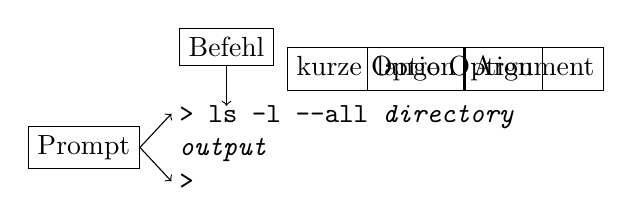
\begin{tikzpicture}
          \node (text) [inner sep=0mm,outer sep=0mm,anchor=west,align=left] at (0,0) {\texttt{> ls -l --all \textit{directory}}\\
                                                                                      \texttt{\textit{output}}\\
                                                                                      \texttt{> }};
          \node (prompt) [left=5mm,draw,rectangle] at (text.west) {Prompt};
          \draw [->] (prompt.east) to ($(text.north west) - (0.1,0.1)$);
          \draw [->] (prompt.east) to ($(text.south west) - (0.1,-0.1)$);
          \node (command) [anchor=south,draw,rectangle] at ($(text.north west) + (0.6,0.5)$) {Befehl};
          \draw [->] (command.south) to ($(text.north west) + (0.6,0)$);
          \node (short) [draw,rectangle] at (2.5,1) {kurze Option};
          \node (long) [draw,rectangle] at (3.5,1) {lange Option};
          \node (argument) [draw,rectangle] at (4.5,1) {Argument};
        \end{tikzpicture}
      \end{frame}
      \begin{frame}{Allgemeines}
        pipes\\
        ctrl-c\\
        ctrl-d\\
        .., .\\
        >, >>, <\\
        glob (*, ...)
      \end{frame}
    \subsection{Befehle}
      \begin{frame}{man}
      \end{frame}
      \begin{frame}{cd, mkdir, pwd}
        mkdir -p
      \end{frame}
      \begin{frame}{ls}
        ls -l\\
        ls -a\\
        ls -R
      \end{frame}
      \begin{frame}{cp, mv, rm}
        cp -r\\
        rm -r\\
        rm -f
      \end{frame}
      \begin{frame}{cat, less}
      \end{frame}
      \begin{frame}{grep}
      \end{frame}
  \section{git}
    \subsection{Allgemeines}
      \begin{frame}{warum}
      \end{frame}
      \begin{frame}{hoster}
      \end{frame}
    \subsection{Befehle}
      \begin{frame}{init, clone}
      \end{frame}
      \begin{frame}{status, log}
      \end{frame}
      \begin{frame}{add, mv, rm}
      \end{frame}
      \begin{frame}{commit}
      \end{frame}
      \begin{frame}{push, pull}
      \end{frame}
      \begin{frame}{mergetool}
      \end{frame}
  \section{Python}
    \begin{frame}
    \end{frame}
    \subsection{Sprache}
      \begin{frame}{ipython}
      \end{frame}
      \begin{frame}{variablen, operatoren}
      \end{frame}
      \begin{frame}{(), [], \{\}}
      \end{frame}
      \begin{frame}{if, elif, else}
      \end{frame}
      \begin{frame}{for, while}
      \end{frame}
      \begin{frame}{def, funktionsaufruf}
      \end{frame}
      \begin{frame}{import, from, as}
      \end{frame}
    \subsection{Bibliotheken}
      \begin{frame}{numpy}
      \end{frame}
      \begin{frame}{scipy}
      \end{frame}
      \begin{frame}{matplotlib}
      \end{frame}
      \begin{frame}{uncertainties}
      \end{frame}
      \begin{frame}{pylab}
      \end{frame}
\end{document}
